\documentclass[a4paper]{article}

\usepackage{hyperref}
%\hypersetup{
%colorlinks=false,              % bool: Liens colorés
%pdfborder={0 0 0}             % Ne pas encadrer les liens
%}
\usepackage[utf8]{inputenc}  
\usepackage[francais]{babel}  
\usepackage[top=2cm, bottom=2cm, left=2cm, right=2cm]{geometry}
\usepackage{graphicx}
\usepackage[final]{pdfpages} 
\usepackage{rotating}
\usepackage{eurosym}
\usepackage{lscape}
\usepackage{float}
% définir les commandes ici

% s'il y a beaucoup de commandes et de packages à inclure n'h&ésitez pas
% à mettre tout ça dans un fichier include.tex et l'inclure
% \input{include.tex}


\begin{document}

%------------------------------------- Page de titre
\begin{titlepage}
~ 
\vfill
	\begin{center}
		\begin{Huge}
		SOA : Dossier de conception détaillée\\
		\end{Huge} 
\vfill
		\textbf{Hexanome 4211 :} 
		\\Sandra \bsc{Mondain}, Elisa \bsc{Abidh}, 
		\\Gaël \bsc{Motte}, Armand \bsc{Rossius}, 
		\\Rémi \bsc{Fradet}, Nicolas \bsc{Silva}, Julien \bsc{Levesy}\\

\vfill		
		\begin{Large}
		Avril 2011
		\end{Large}
\vfill
	\begin{tabular}{|c|c|c|c|c|}
 	 \hline
 	 Auteur du Document & Responsable Validation & Phase & Etat & Avancement \\
 	 \hline
 	 
 	\hline
 	
	\end{tabular}
\vfill	
	\end{center}
\vfill
\end{titlepage}
%----------------------------------------------------

%--------------------------------- Table des matières
\newpage
\tableofcontents
\newpage
%----------------------------------------------- Plan


\section*{Introduction}
blah

\section{Diagrammes d'Enchainement des Fenêtres}

\subsection{Diagramme d'enchainement des Fenêtre - Client} 

\begin{figure}[H]
	\begin{center}
		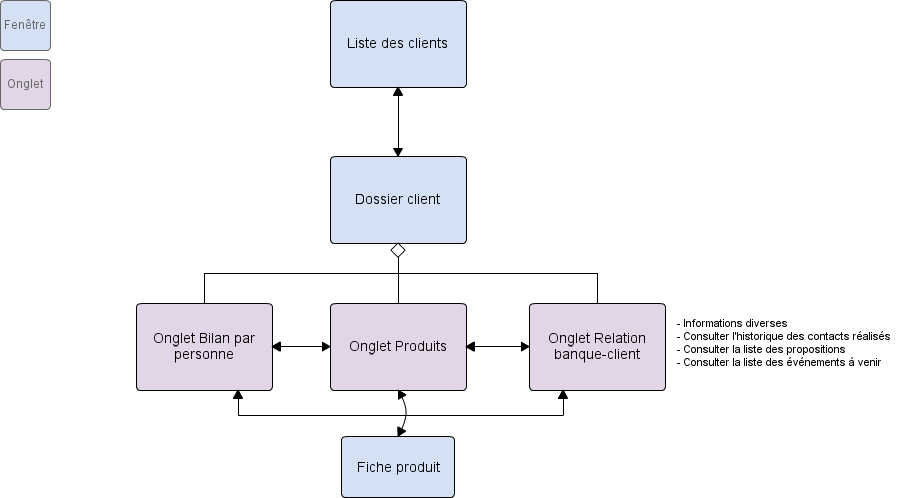
\includegraphics[scale=0.6]{EDF/Client.png}
		\caption{Diagramme d'enchainement des Fenêtre - Client}
	\end{center}
\end{figure}

\subsection{Diagramme d'enchainement des Fenêtre - Contact} 

\begin{figure}[H]
	\begin{center}
		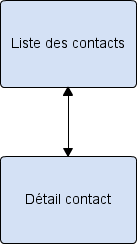
\includegraphics[scale=0.6]{EDF/Contact.png}
		\caption{Diagramme d'enchainement des Fenêtre - Client}
	\end{center}
\end{figure}

\subsection{Diagramme d'enchainement des Fenêtre - Agenda} 

\begin{figure}[H]
	\begin{center}
		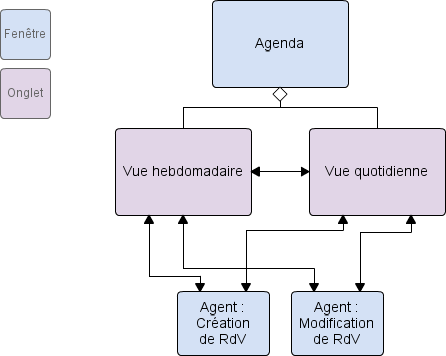
\includegraphics[scale=0.6]{EDF/Agenda.png}
		\caption{Diagramme d'enchainement des Fenêtre - Client}
	\end{center}
\end{figure}
\section{Maquettes de l'IHM} 

	\subsection{Client}
	
		\subsubsection{Liste des clients}
		Cette fenêtre permet de consulter la liste des clients de l'agence et d'effectuer des recherches dans cette liste. Au double-clic sur une ligne, une fenêtre contenant le dossier client correspondant s'ouvre. \\
		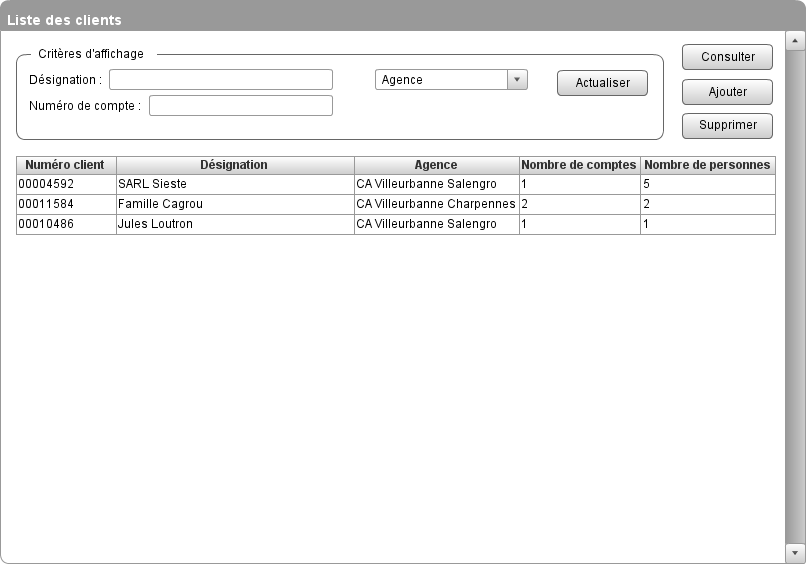
\includegraphics[width=\linewidth]{IHM/Liste_Clients.png}
		
		\newpage		
		
		\subsubsection{Dossier client}
		Lorsque l'on ouvre un dossier client, on accède à ses informations générales (situées en haut de la page). La page contient également 3 onglets : bilan par personne, produits et relation banque-client. Par défaut le premier onglet est sélectionné. \\
		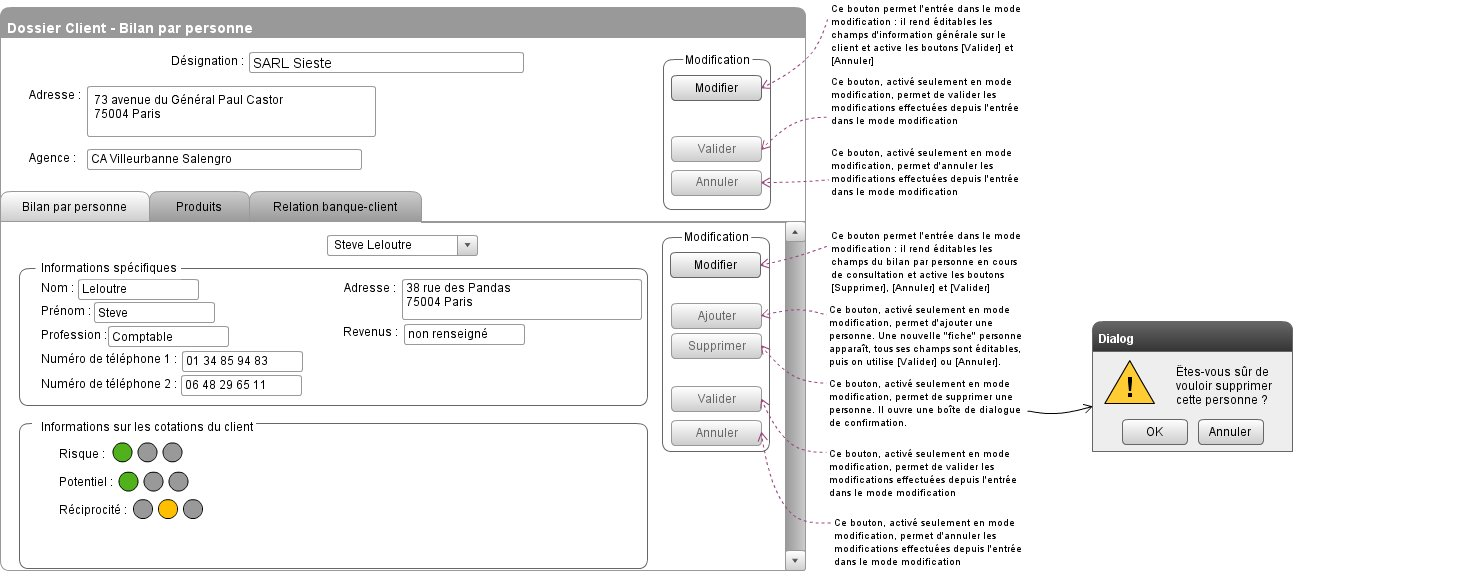
\includegraphics[scale=0.45, angle=90]{IHM/IHMclient1.jpg}
		
		\paragraph*{}
		Ce schéma montre le deuxième onglet. \\
		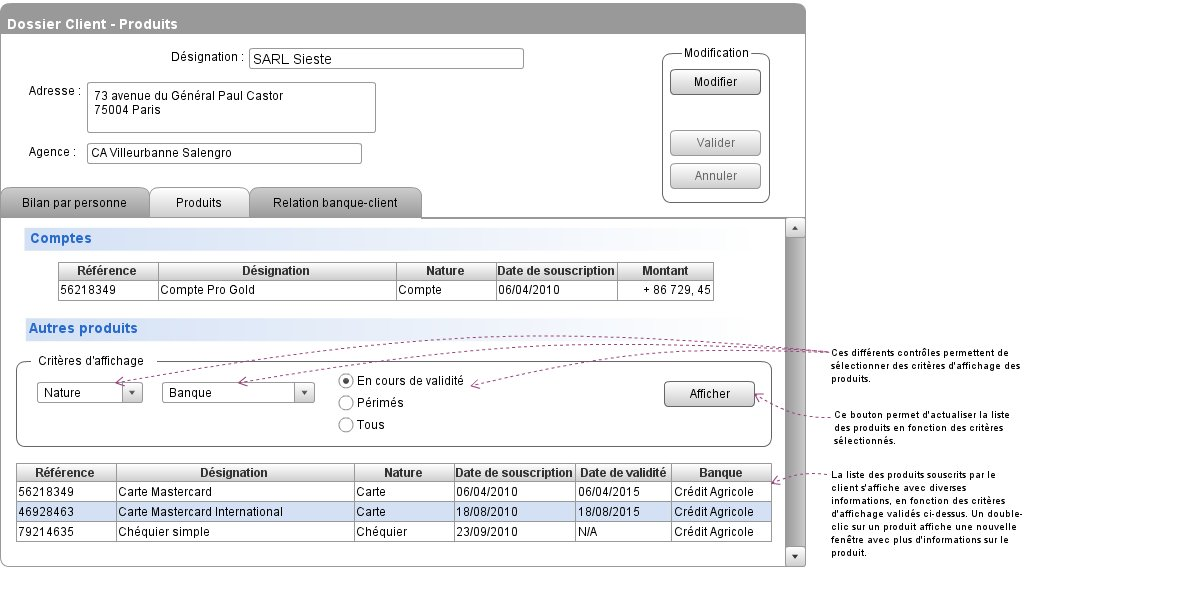
\includegraphics[width=\linewidth]{IHM/IHMclient2.jpg}
		
		\paragraph*{}
		Ces 4 schémas montrent le troisième onglet, qui contient un menu avec 4 options. \\
		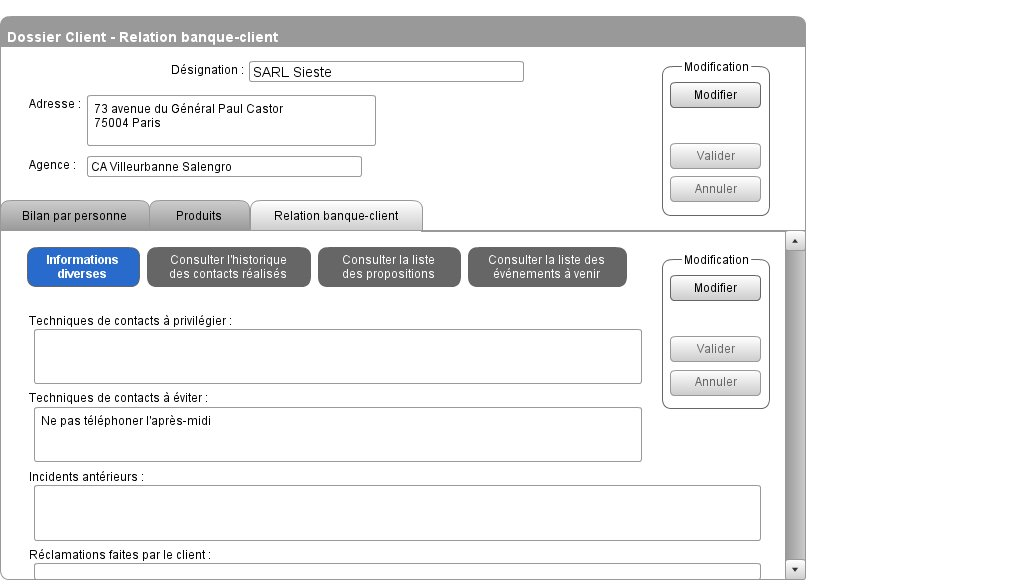
\includegraphics[width=\linewidth]{IHM/IHMclient3.jpg} \\
		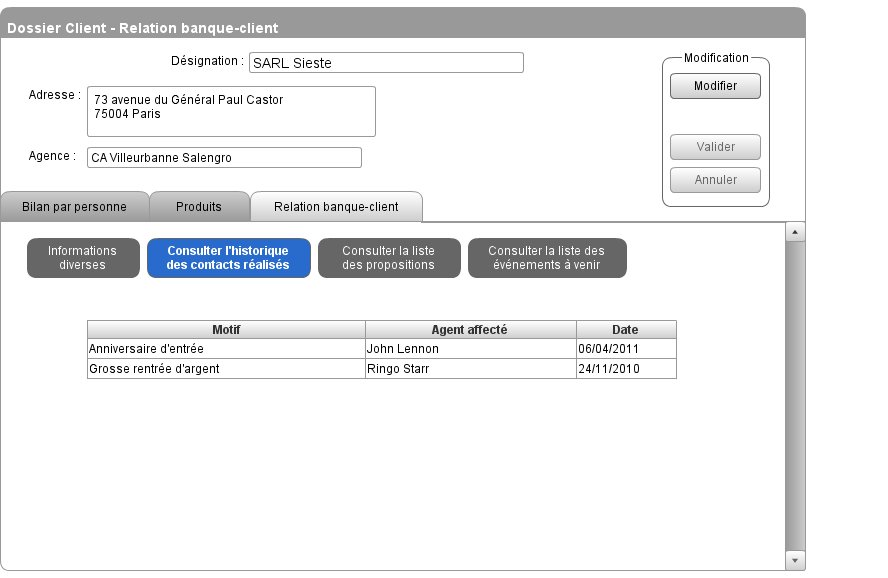
\includegraphics[width=\linewidth]{IHM/IHMclient4.jpg} \\
		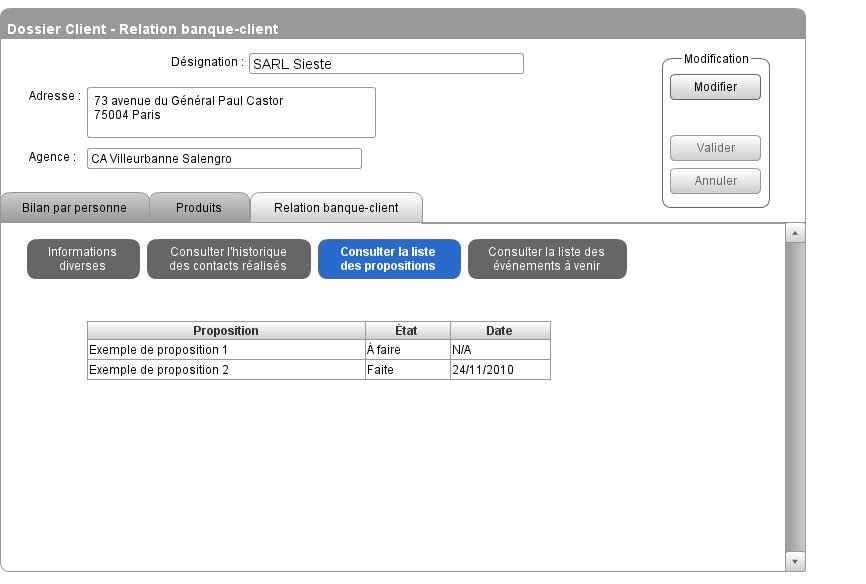
\includegraphics[width=\linewidth]{IHM/IHMclient5.jpg} \\
		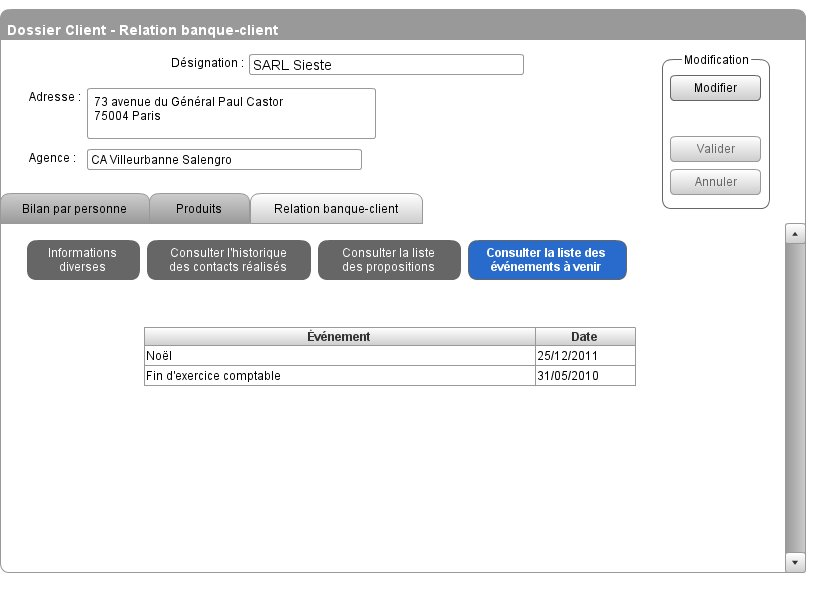
\includegraphics[width=\linewidth]{IHM/IHMclient6.jpg} 
		
	\newpage
		
	\subsection{Contact}
	
		\subsubsection{Liste des contacts}
		Cette fenêtre permet de consulter la liste des contacts de l'agence et d'effectuer des recherches dans cette liste. Au double-clic sur une ligne, une fenêtre contenant les détails du contact correspondant s'ouvre. \\
		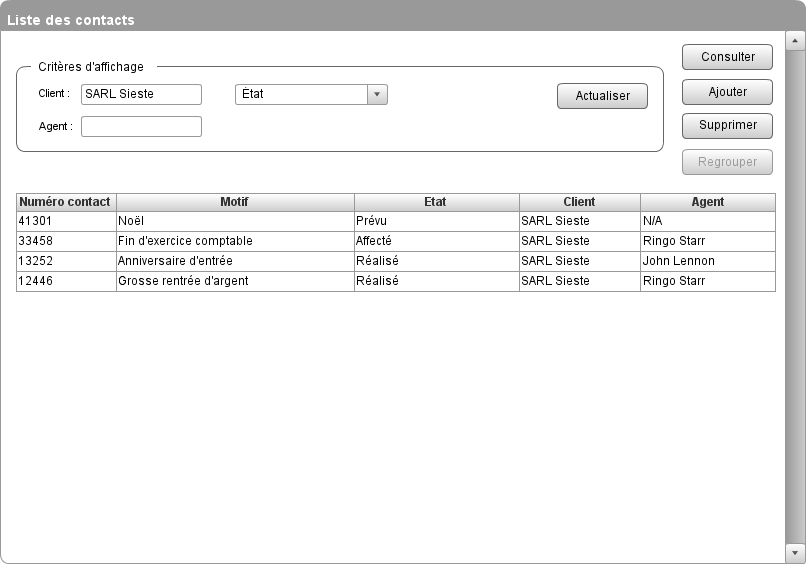
\includegraphics[width=\linewidth]{IHM/Liste_Contacts.png}
		
		\subsubsection{Détail d'un contact}
		Cette fenêtre permet de consulter les détails d'un contact. \\
		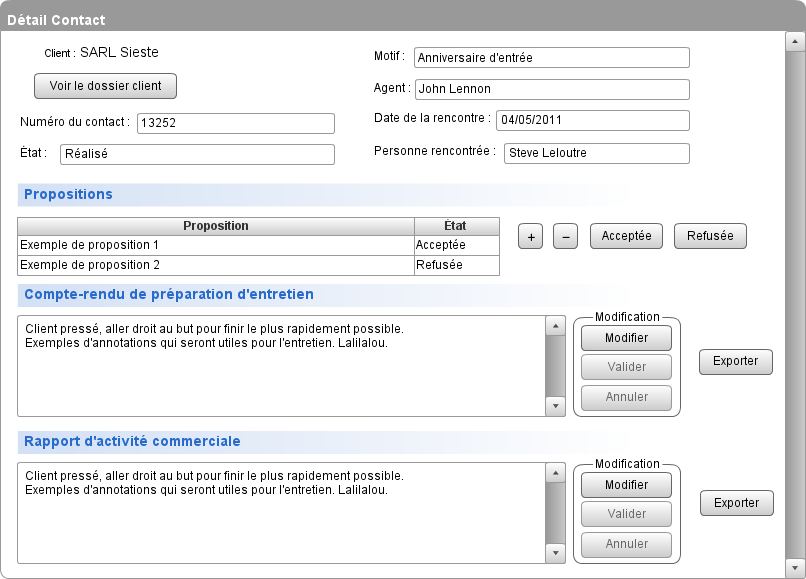
\includegraphics[width=\linewidth]{IHM/Detail_Contact.png}
		
		\newpage
		
	\subsection{Agenda}
		Cette fenêtre permet de consulter l'agenda des agents de l'agence, de créer des plages agenda, de prendre des rendez-vous, de les modifier ou les annuler. \\
		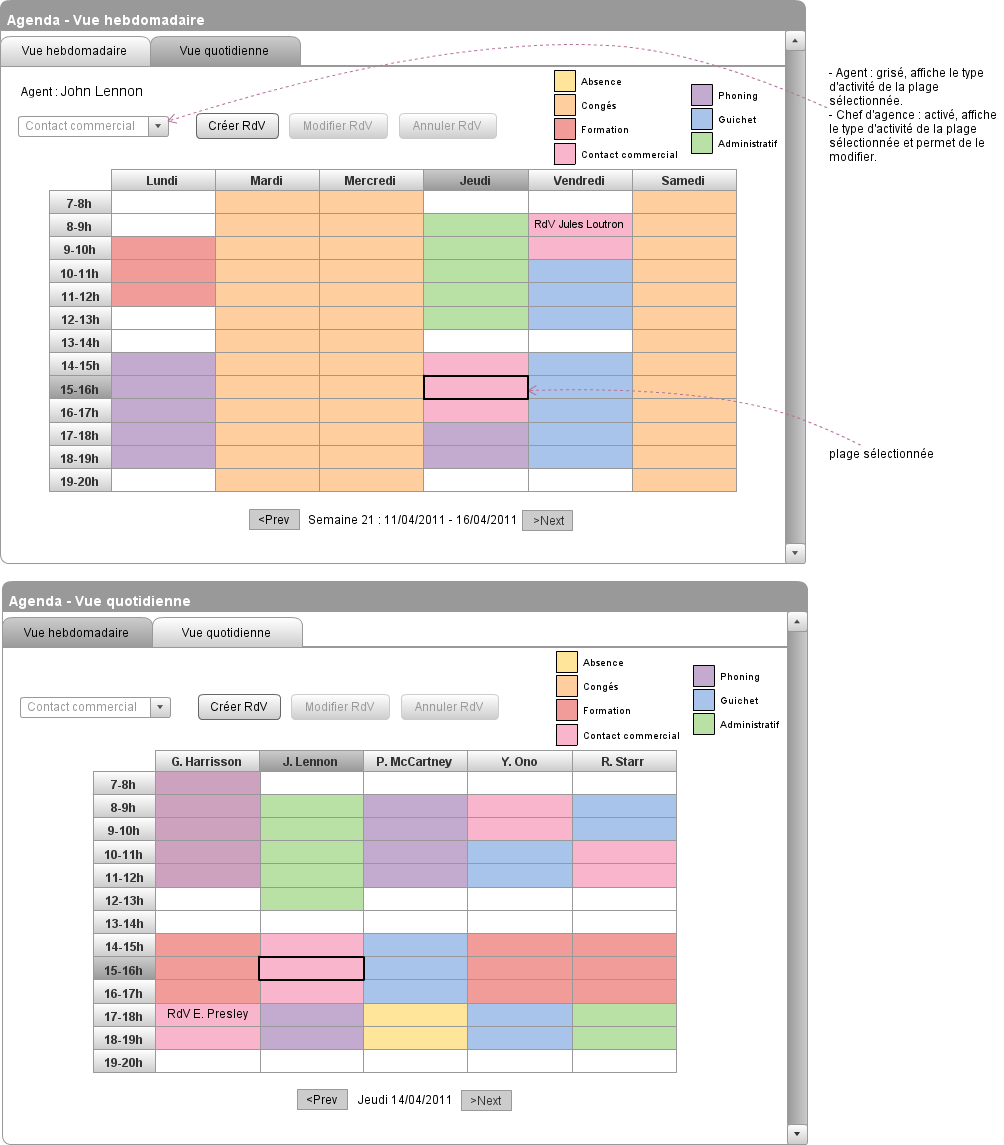
\includegraphics[width=\linewidth]{IHM/Agenda.png}
		
		\newpage
\section{Listes des services}
\subsection{IHM Client}
\subsubsection*{Informations générales}
\begin{itemize}
\item ConsulterInfosClient
\item ModifierInfosClient
\end{itemize}
\subsubsection*{Bilan par personne}
\begin{itemize}
\item ConsulterBilan 
\item ModifierBilan 
\item AjouterPersonne 
\item SupprimerPersonne
\end{itemize}
\subsubsection*{Produit}
\begin{itemize}
\item ConsulterComptesClient 
\item AfficherProduits 
\item SelectionnerProduit 
\item ConsulterFicheProduit
\end{itemize}

\subsubsection*{Relation banque client}
\begin{itemize}
\item ConsulterInfos
\item ConsulterHistoriqueContacts  
\item ConsulterPropositions 
\item ConsulterEvénements 

\end{itemize}


\end{document}
